% !TEX root = ./physics.tex

\chapter{Nature of Light}
	
\section{Introduction}
	
	\subsection{Maxwell's Equations}
	
		Gauss' Law (1813) $\rightarrow$ Electric flux ($\Phi_E = E \times \Delta A$) of any closed surface.

		Electric flux is defined as the electric field (E) times the component of the area perpendicular to the field.

		The area integral of the electric field over any closed surface is equal to the net charge divided by the permittivity of free space.

		Gauss' Law of Magnetism

		The net magnetic flux out of any enclosed surface is zero

		For any magnetic dipole, any magnetic flux directed inward toward the south pole will equal the flux outward from the north pole

		There are no magnetic monopoles

		Ampere's Law (1826)

		Describes the magnetic field around a closed conductor loop to the strength of the electric current flowing through the loop

		A changing magnetic field creates a changing electric field
		A changing electric field creates a changing magnetic field

		This means that they can like propagate each other


		Hertz's Experiment

		Maxwell predicted there would be other forms of electromagnetic waves - that light was just one example

\newpage

\section{Practical Investigation - Estimating the speed of light}

	\subsection{Introduction}
	
		Using the equation $v = f \lambda$ to determine the speed of light

		The microwave is designed such that microwaves are reflected off the opposite wall to create a standing wave. This causes fluctuations in energy depending on the point of the wave (at the maximums). The wavelength can be determined by measuring the distance between each gap in the chocolate.

		Accuracy can be improved by minimising size of holes. The size of the microwaves is small, so larger holes will create significant error

	\textbf{Aim}: To estimate the speed of light

	\subsection{Materials}
	
		\begin{itemize}
			\item Large chocolate block
			\item Microwave (frequency of 2450 MHz)
		\end{itemize}

	\subsection{Risk Assessment}
		\begin{table}[H]
			\centering
			\begin{tabular}{p{7cm}|p{7cm}}
				Hazard & Precaution \\ \hline
				Burning from hot chocolate & Wear oven mitts when removing the chocolate and allow adequate cooling before handling \\
				Dropping parts of the microwave & Handle the baseplate of the microwave with caution
			\end{tabular}
		\end{table}

	\subsection{Method}
	
		\begin{enumerate}
			\item Prepare a 
		\end{enumerate}

\section{Spectroscopy} \label{08/05/2025}
	
	\subsection{Star Analysis}
	
		The qualities of stars can be predicted by observing their colours. Different temperatures emit different levels of visible light

\newpage

\section{Analysis of Star Spectra}

	\subsection{}

	A star's inner nucleus produces a light source that contains a continuous spectrum of all wavelengths, with a peak at a certain point depending on the temperature of the star.

	Stars are made of a ball of gas that varies the colour emitted by the star as a whole. This is due to fluctuation in energy levels of atoms, exciting electrons within these atoms and allowing electrons to "jump" to another orbital level. The electrons in the excited state absorb specific wavelengths of light, and create gaps in the light spectrum after passing through the gas.

	The excited electrons will also fall, emitting energy and also providing information about the star. Hence, the composition profile of the star's gas can be determined using it's emission spectrum (with peaks) or it's absorption spectrum (with dips in the full spectrum).

	\subsection{Spectroscope}
	
		A spectroscope is a device used to display the absorption spectrum of a given element

		High voltage is passed through a tube containing a particular element. The light emitted by the gas is passed through a prism to separate the wavelengths and projected onto a screen. This can be used to analysis the chemical composition of the star, as well as other physical properties.

		\subsubsection{Analysis of the Absorption Spectrum}
		
			\begin{itemize}
				\item Rotational velocity
					\begin{itemize}
						\item As the star rotates, the light is blue or red shifted. This creates wider lines on the absorption spectrum as the rotational velocity increases
					\end{itemize}

				\item Translational velocity
					\begin{itemize}
						\item Due to movement towards and away from a fixed point, the entire light spectrum can either be blue or red shifted
						\item All the lines on the spectrum are shifted equally depending on the relative velocity of the star
						\item By using the known properties of elements (commonly hydrogen), the spectrum can be compared to that of one where the star was not moving
					\end{itemize}

				\item Density
					\begin{itemize}
						\item If the star is made of high density gas, more collisions occur between the atoms and further the electrons
						\item These collisions vary the energy that the electron has as it moves between orbital states, creating small variations of wavelength produced
						\item This variation is depicted on the spectrum as a blurred line
					\end{itemize}
				
				\item Chemical composition
					\begin{itemize}
						\item Different chemicals produce different emissions spectra
						\item A star will emit multiple overlapping spectra that form the spectrum that is visible from an external observer
					\end{itemize}
			\end{itemize}

\section{Diffraction and Interference} \label{15/05/2025}
	
	Diffraction is the spreading out of a waves when it passes a barrier or small opening. The size of the obstacle should be the same order of magnitude as the wavelength.

	Interference occurs when two waves reach a point at the same time, causing the waves to combine either constructively or destructively

	Chromatic light contains many wavelengths of light, however interference can only be observed when the light is monochromatic and in phase. The best way to achieve this is by a laser.

	\subsection{Young's Double Slit Experiment}
	
		In order for the two-slit interference pattern to result, the light hitting the double slit should be monochromatic and coherent. $d$ is the separation of the double slits, $S_{2}M - S_{1}M$ is the path difference, $L$ is the distance between the double slits to the screen, and $x$ is the distance from the central maximum to position $M$.

		The central maximum is always a bright fringe.

		The first minimum is produced when the wave from $S_1$ has travelled one half of a wavelength further than the save from $S_2$. When $S_1 C - S_2 C = \lambda$, the area is brighter.

		\begin{figure}[H]
			\centering
			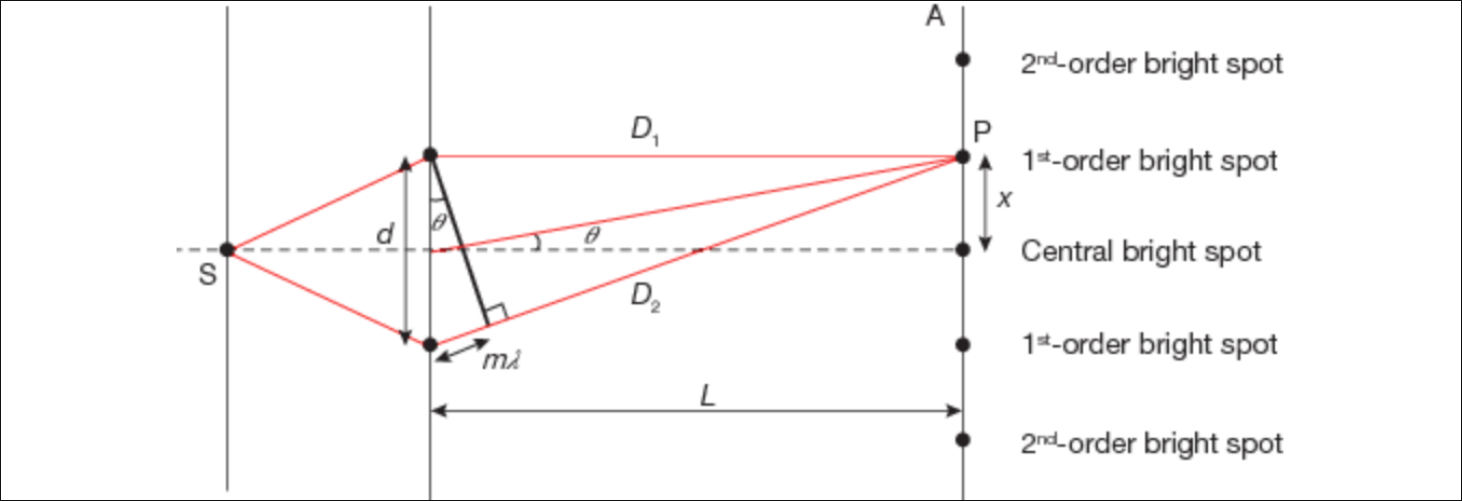
\includegraphics[width=15cm]{young_double_slit.png}
		\end{figure}

	
